\documentclass[11pt,a4paper]{article}
\usepackage[utf8]{inputenc}
\usepackage[T1]{fontenc}
\usepackage[french]{babel}
\usepackage{geometry}
\geometry{margin=2.5cm}
\usepackage{booktabs}
\usepackage{listings}
\usepackage{graphicx}

\title{Journal de bord -- Projet 2 partie 1\\HAI716I}
\author{Neha HAJEE}
\date{}

\begin{document}

\maketitle

\section{Organisation du binôme}
L'énoncé indique un travail individuel, mais le travail en binôme a été autorisé oralement par le professeur, avec une
répartition libre des tâches. Le binôme est composé de Neha HAJEE et Zéinab CAMARA.

Le travail a été séparé en deux parties qui communiquent par un contrat commun, la classe \texttt{Strategie}.
L'étape 0, c'est-à-dire la définition de l'interface entre le moteur et les stratégies et les décisions de protocole, a été
faite ensemble. Pour l'étape 1, Neha HAJEE s'est chargée du moteur (\texttt{moteur.py}), qui comprend une partie entre deux
stratégies, le tournoi tous contre tous, le calcul des scores, le classement et la gestion de la graine, ainsi que du lancement
(\texttt{main.py}) et du README. Zéinab s'est chargée des stratégies (\texttt{strategies.py}), c'est-à-dire des cinq stratégies
du cours (ALL-D, RANDOM, TIT-FOR-TAT, TESTER et JOSS), de leurs tests à partir des valeurs du cours et de la question sur la
victoire de TIT-FOR-TAT. Pour les étapes 2 et 3, chacune ajoute au moins une nouvelle stratégie et prend en charge une
modification du tournoi.

Cette répartition permet de travailler en parallèle. Tant que le contrat est respecté, le moteur n'a pas besoin de connaître
le détail des stratégies, et les stratégies n'ont pas besoin de savoir comment le moteur fonctionne. Chacune tient son propre
journal de bord, mais les décisions de protocole sont prises ensemble et sont identiques dans les deux journaux.

\section{Étape 0 -- Contrat entre moteur et stratégies}
\subsection{Interface de la classe Strategie}
Toutes les stratégies ayant la même forme, la décision a été prise de modéliser une classe mère \texttt{Strategie}. Le moteur
peut donc les faire jouer sans savoir laquelle est en face. La classe contient un nom et deux méthodes, \texttt{reset} et
\texttt{jouer}. Le nom est une chaîne de caractères qui permet de reconnaître chaque stratégie dans le classement. Il est
obligatoire et n'a donc pas de valeur par défaut.

La méthode \texttt{reset} est appelée par le moteur au début de chaque partie. Elle permet aux stratégies qui ont une mémoire
interne d'effacer cette mémoire, afin que la partie précédente ne fausse pas la suivante. Elle contient seulement le mot clé
\texttt{pass}, car ne rien faire est un comportement par défaut correct pour les stratégies sans mémoire.

La méthode \texttt{jouer} est appelée par le moteur à chaque tour. Elle reçoit la liste de ses propres coups, la liste des coups
de l'adversaire et le générateur aléatoire \texttt{rng}, et renvoie le coup joué. Elle lève l'exception
\texttt{NotImplementedError}, car il n'existe pas de coup par défaut raisonnable. Si une stratégie oublie de la redéfinir, le
programme doit s'arrêter avec une erreur plutôt que de jouer un coup faux sans prévenir.

\subsection{Décisions de protocole}
\paragraph{Paramètres imposés par l'énoncé.} Le tournoi suit le format d'Axelrod. Chaque stratégie affronte chaque autre sur
5 parties de 200 tours, et le meilleur score total gagne. Les gains sont ceux du cours, 3/3 si les deux coopèrent, 0/5 et 5/0
si l'un trahit l'autre, 2/2 si les deux trahissent.

\paragraph{Représentation des coups.} Un coup est représenté par la chaîne \texttt{"C"} ou \texttt{"D"}, comme dans le cours,
ce qui rend les historiques faciles à lire et à afficher. L'historique est une liste triée du plus ancien au plus récent, le
dernier coup de l'adversaire est donc le dernier élément de la liste. Les listes sont vides au premier tour, ce qui permet à une
stratégie de savoir qu'elle commence. Les listes appartiennent au moteur et les stratégies ne doivent pas les modifier.

\paragraph{Hasard et graine.} Les stratégies qui ont besoin de hasard (RANDOM, JOSS) utilisent uniquement le générateur
\texttt{rng} fourni par le moteur, jamais directement le module \texttt{random}. Une seule graine, fixée à 42, contrôle ainsi
tout le tournoi, et les résultats peuvent être relancés à l'identique, comme l'exige l'énoncé.

\paragraph{Une stratégie joue-t-elle contre elle-même ?}
Une stratégie ne joue pas contre elle-même, mais elle a le droit de jouer contre un autre joueur possédant la même stratégie.
Cette décision a été prise pour ne pas avantager les stratégies coopératives, car un match de TIT-FOR-TAT contre sa propre copie
rapporterait 600 points par partie, contre 400 pour ALL-D. C'est aussi ce que fait le mini-tournoi du cours, où un joueur
n'affronte jamais lui-même. Le moteur propose toutefois une option \texttt{--auto-play} qui active ces matchs, afin de pouvoir
comparer avec le tournoi d'Axelrod de 1980, où chaque stratégie affrontait aussi sa propre copie.

\paragraph{TESTER, qu'est-ce qu'une riposte ?}
Une riposte est une réponse à une trahison par une trahison. Seul le coup de l'adversaire au tour 2 est pris en compte, car
c'est sa réponse directe à la trahison de TESTER au tour 1. Si ce coup est D, TESTER joue TIT-FOR-TAT pour le reste de la
partie, sinon il répète C, C, D jusqu'à la fin. La décision est prise une seule fois et gardée pour toute la partie, ce qui
suit la règle du cours mot pour mot et reste simple à tester. Ce choix a une limite, puisque contre RANDOM la décision dépend
d'un seul tirage au hasard, celui du tour 2.

\paragraph{JOSS, \og une fois sur dix \fg{}, probabilité ou compteur ?}
Chaque fois que JOSS devrait jouer C, il tire au sort et joue D avec une probabilité de 10~\%. Le nombre de trahisons varie
donc d'une partie à l'autre, et le hasard passe par \texttt{rng}. Cette option correspond mieux à l'esprit d'un tricheur
imprévisible qu'un compteur régulier.

\paragraph{Ex aequo dans le classement.}
Lorsque deux stratégies ont exactement le même score total, celle qui vient en premier dans l'ordre alphabétique est classée
devant, afin de garantir un affichage stable d'une exécution à l'autre.

\section{Étape 1 -- Tournoi de base}
\subsection{Moteur}
\paragraph{Objectif.} Le moteur doit faire jouer une partie entre deux stratégies, puis un tournoi tous contre tous, sans
connaître le détail des stratégies. Il ne passe que par les méthodes \texttt{reset} et \texttt{jouer} définies à l'étape 0.

\paragraph{Matrice des gains.} Elle est représentée par un dictionnaire dont la clé est le couple de coups (coup du joueur 1,
coup du joueur 2) et la valeur le couple de gains correspondant. Par exemple, \texttt{("C", "D")} donne \texttt{(0, 5)}. Le
gain d'un tour s'obtient ainsi en une seule lecture.

\paragraph{Déroulement d'une partie.} La fonction \texttt{jouer\_partie} remet les deux stratégies à zéro avec \texttt{reset},
puis, à chaque tour, demande son coup à chaque stratégie, vérifie ces coups, les ajoute aux historiques et ajoute les gains
aux scores. Elle renvoie les deux scores de la partie.

\paragraph{Choix de conception.} Trois choix ont été faits lors de l'écriture de \texttt{jouer\_partie}. Le premier concerne la
simultanéité des coups. Les deux coups sont demandés avant d'être ajoutés aux historiques, si bien qu'aucune stratégie ne peut
voir le coup de l'adversaire du tour en cours. Cela respecte la règle de l'énoncé, selon laquelle les deux joueurs choisissent
\og en même temps \fg{}.

Le deuxième choix est la copie des historiques. Chaque stratégie reçoit une copie des listes et non les listes du moteur.
Une stratégie qui modifierait sa liste par erreur ne peut donc pas fausser la partie. Le moteur fait ainsi respecter le contrat
de l'étape 0 au lieu de simplement faire confiance aux stratégies.

Le troisième choix est la vérification des coups. Si une stratégie renvoie autre chose que \texttt{"C"} ou \texttt{"D"}, le
moteur lève une erreur (\texttt{ValueError}) dont le message donne le nom de la stratégie et le coup reçu. Sans cette
vérification, le programme planterait plus loin, lors de la lecture des gains, avec un message beaucoup moins clair.

\paragraph{Vérification.} Pour contrôler \texttt{jouer\_partie} avant que les stratégies du cours soient écrites, la fonction a
été lancée sur 200 tours avec deux stratégies très simples, l'une jouant toujours C et l'autre toujours D, dont les scores se
calculent à la main.
\begin{center}
\begin{tabular}{lcc}
\toprule
Partie & Attendu & Obtenu \\
\midrule
toujours C contre toujours D & (0, 1000) & (0, 1000) \\
toujours D contre toujours D & (400, 400) & (400, 400) \\
toujours C contre toujours C & (600, 600) & (600, 600) \\
\bottomrule
\end{tabular}
\end{center}
Les résultats obtenus correspondent aux valeurs attendues, la lecture de la matrice et le calcul des scores sont donc
corrects. Une stratégie renvoyant \texttt{"X"} provoque bien l'erreur attendue.

\paragraph{Match.} La fonction \texttt{jouer\_match} fait jouer deux stratégies sur plusieurs parties (5 au format d'Axelrod)
et additionne les scores de chaque partie. Elle n'a pas besoin d'appeler \texttt{reset}, puisque \texttt{jouer\_partie} le
fait déjà au début de chaque partie, ce qui garantit que les parties sont indépendantes.

\paragraph{Tournoi.} La fonction \texttt{tournoi} crée un score total à 0 pour chaque stratégie, puis fait jouer un match à
chaque paire de stratégies et ajoute les points obtenus au total de chacune. Les paires sont générées avec
\texttt{itertools.combinations}. Ainsi, chaque paire ne se rencontre qu'une seule fois (A contre B, mais pas en plus B contre
A), et aucune stratégie n'affronte elle-même. La fonction renvoie aussi le détail de chaque match, qui sert à expliquer le
classement en montrant contre qui une stratégie gagne ou perd des points.

\paragraph{Option auto play.} Lorsque l'option est activée, les paires sont générées avec
\texttt{itertools.combinations\_with\_replacement}, qui ajoute les paires (A, A). Deux points ont demandé une attention
particulière. D'abord, si le même objet jouait des deux côtés, les stratégies qui ont une mémoire interne partageraient cette
mémoire entre les deux joueurs. Le second joueur est donc une copie indépendante, créée avec \texttt{copy.deepcopy}.

Ensuite, dans un match A contre A, les deux scores reviennent au même nom. Seul le score d'un des deux joueurs est ajouté,
sinon la stratégie recevrait les points de deux joueurs. Ce choix a une limite. Pour une stratégie aléatoire (RANDOM, JOSS),
les deux copies n'obtiennent pas le même score, et ce choix revient à garder l'une des deux.

\paragraph{Classement.} La fonction \texttt{classement} trie les stratégies par score total décroissant, puis par ordre
alphabétique en cas d'égalité, comme décidé à l'étape 0. Le tri se fait sur le couple (score négatif, nom). Le signe moins
permet d'obtenir l'ordre décroissant pour le score tout en gardant l'ordre alphabétique croissant pour le nom.

\paragraph{Lancement (\texttt{main.py}).} Le tournoi se lance avec \texttt{python3 main.py}. Les options \texttt{--graine},
\texttt{--tours}, \texttt{--parties} et \texttt{--auto-play} ont pour valeurs par défaut celles du protocole. Le générateur
aléatoire est créé une seule fois à partir de la graine, puis transmis à tout le tournoi. Le classement est affiché avec les
paramètres utilisés et exporté dans un fichier CSV dont le nom contient la graine, afin de garder une trace de chaque lancement
sans écraser les précédents.

\paragraph{Vérification du tournoi.} Le tournoi a été lancé avec trois stratégies simples, deux stratégies jouant toujours C
(C1 et C2) et une jouant toujours D, sur 5 parties de 200 tours.
\begin{center}
\begin{tabular}{lcccc}
\toprule
 & Matchs & C1 & C2 & D \\
\midrule
Sans auto play (attendu) & 3 & 3000 & 3000 & 10\,000 \\
Sans auto play (obtenu) & 3 & 3000 & 3000 & 10\,000 \\
Avec auto play (attendu) & 6 & 6000 & 6000 & 12\,000 \\
Avec auto play (obtenu) & 6 & 6000 & 6000 & 12\,000 \\
\bottomrule
\end{tabular}
\end{center}
Sans auto play, D bat C1 et C2 (5000 points chacun) et C1 et C2 coopèrent entre eux (3000 chacun). Avec auto play, chaque
stratégie gagne en plus son match contre sa copie, 3000 pour C1 et C2, mais seulement 2000 pour D. Ce résultat montre déjà que
l'auto play avantage les stratégies coopératives. Pour le classement, des scores fictifs (TFT 9900, ALL-D 9500, JOSS 9000,
AAA 9000) donnent bien l'ordre TFT, ALL-D, AAA, JOSS, trié par score puis par ordre alphabétique pour les ex aequo. Enfin, deux
tournois lancés avec la graine 42 donnent exactement les mêmes scores, et la graine 7 donne des scores différents, ce qui
montre que les résultats sont reproductibles.

\subsection{Tests}
%les tests des stratégies sont décrits dans le journal de Zéinab
%à faire : capture de la sortie des tests

\subsection{Classement obtenu}
Le tournoi officiel a été lancé avec les cinq stratégies du cours, au format d'Axelrod (5 parties de 200 tours par match),
avec la graine 42 et sans auto play, à l'aide de la commande \texttt{python3 main.py}. Pour vérifier la reproductibilité, la
commande a été lancée deux fois de suite (figure~\ref{fig:classement}).

\begin{figure}[h]
  \centering
  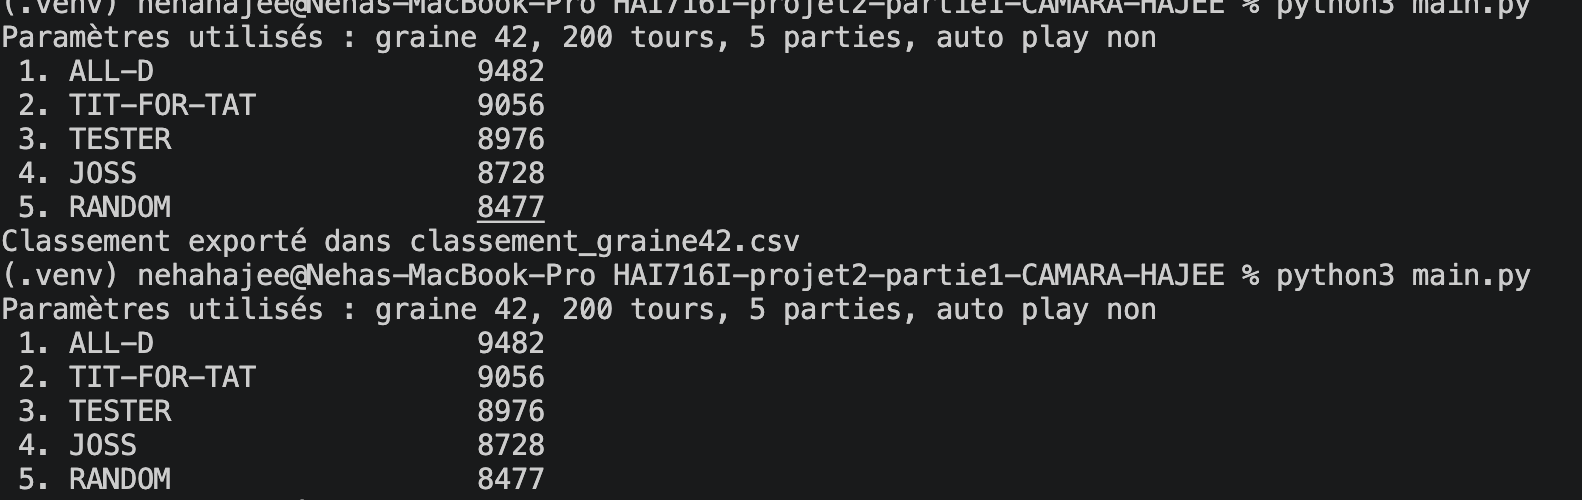
\includegraphics[width=\linewidth]{captures/etape1_classement.png}
  \caption{Deux lancements successifs de \texttt{python3 main.py} (graine 42), le classement est identique.}
  \label{fig:classement}
\end{figure}

\begin{center}
\begin{tabular}{clc}
\toprule
Rang & Stratégie & Score total \\
\midrule
1 & ALL-D & 9482 \\
2 & TIT-FOR-TAT & 9056 \\
3 & TESTER & 8976 \\
4 & JOSS & 8728 \\
5 & RANDOM & 8477 \\
\bottomrule
\end{tabular}
\end{center}

Les deux lancements donnent exactement les mêmes scores, ce qui confirme que la graine contrôle bien tout le hasard du
tournoi. ALL-D termine premier, devant TIT-FOR-TAT. Les écarts restent faibles, environ 1000 points entre le premier et le
dernier, soit moins de 12~\%.

\subsection{TFT gagne-t-il ?}
Avec ce protocole, TIT-FOR-TAT ne gagne pas, il termine deuxième derrière ALL-D. Pour comprendre ce résultat, le détail des
matchs renvoyé par le moteur a été examiné.

\begin{center}
\begin{tabular}{lc}
\toprule
Match & Scores \\
\midrule
ALL-D contre RANDOM & 3440 -- 1040 \\
ALL-D contre TIT-FOR-TAT & 2015 -- 1990 \\
ALL-D contre TESTER & 2015 -- 1990 \\
ALL-D contre JOSS & 2012 -- 1992 \\
RANDOM contre TIT-FOR-TAT & 2497 -- 2487 \\
RANDOM contre TESTER & 2572 -- 2452 \\
RANDOM contre JOSS & 2368 -- 2593 \\
TIT-FOR-TAT contre TESTER & 2500 -- 2500 \\
TIT-FOR-TAT contre JOSS & 2079 -- 2104 \\
TESTER contre JOSS & 2034 -- 2039 \\
\bottomrule
\end{tabular}
\end{center}

La victoire d'ALL-D vient presque entièrement de son match contre RANDOM, qui lui rapporte 3440 points. Contre les trois
autres stratégies, qui ripostent toutes à la trahison, ALL-D ne prend qu'environ 25 points d'avance par match. Sans RANDOM,
TIT-FOR-TAT passerait devant.

La population est aussi trop petite et peu coopérative, comme l'indique la diapositive 69. TIT-FOR-TAT est la seule stratégie
\og gentille \fg{}, c'est-à-dire qui ne trahit jamais en premier. TESTER trahit dès le premier tour, JOSS et RANDOM trahissent
au hasard. Aucun match n'atteint donc la coopération complète (3000 points chacun), alors que c'est précisément ce qui faisait
gagner TIT-FOR-TAT en 1980.

Le détail montre également un effet d'écho. Contre TESTER, le score est exactement de 2500 partout. TESTER trahit au premier
tour, TIT-FOR-TAT riposte, et les deux stratégies se renvoient ensuite la trahison en alternance, soit 2,5 points par tour en
moyenne. Contre JOSS, chaque trahison au hasard déclenche de la même façon une chaîne de représailles. TIT-FOR-TAT ne gagne
d'ailleurs aucun de ses matchs, il termine deuxième parce qu'il ne perd jamais de beaucoup.

Enfin, le protocole diffère de celui de 1980. Le tournoi d'Axelrod comptait 14 participants, majoritairement gentils, et chaque
stratégie affrontait aussi sa propre copie. En relançant le tournoi avec l'option \texttt{--auto-play}
(figure~\ref{fig:autoplay}), TIT-FOR-TAT redevient premier avec 12042 points. Son match contre sa copie lui rapporte la
coopération complète, alors qu'ALL-D ne gagne que 2 points par tour contre la sienne.

\begin{figure}[h]
  \centering
  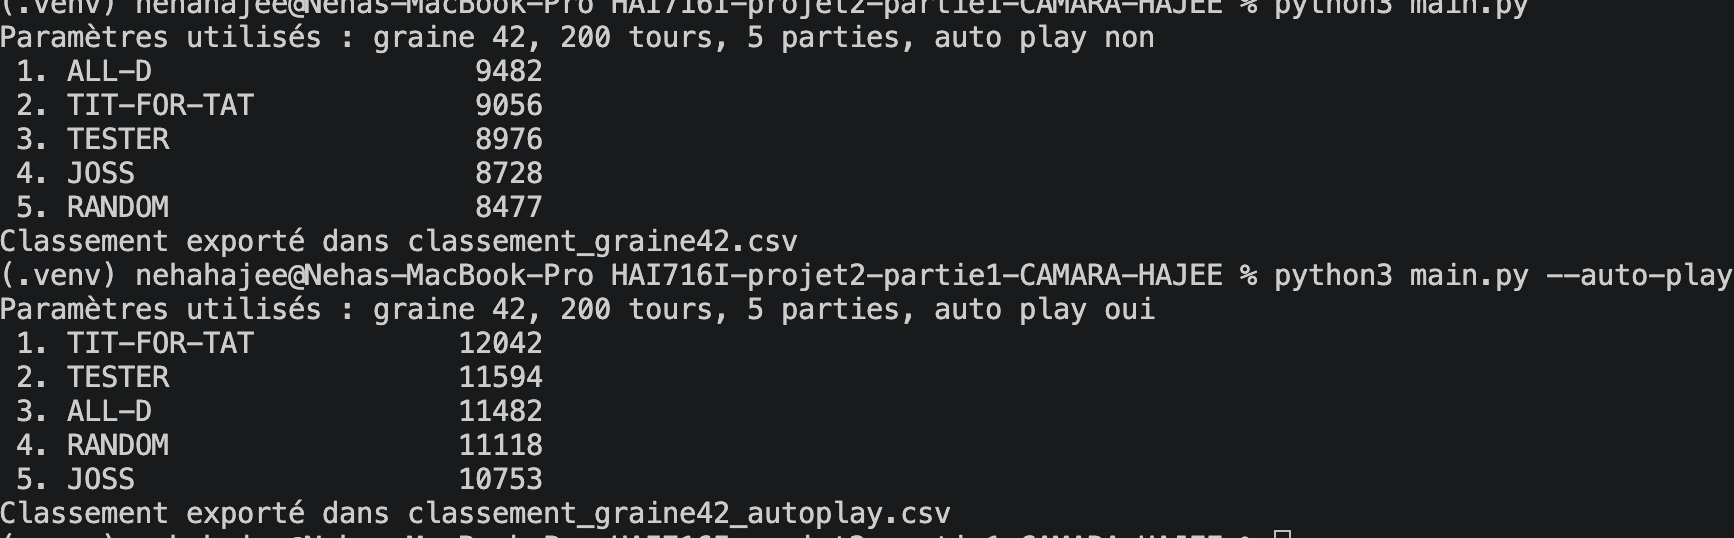
\includegraphics[width=\linewidth]{captures/etape1_autoplay.png}
  \caption{Tournoi sans auto play puis avec auto play (graine 42). TIT-FOR-TAT passe de la deuxième à la première place.}
  \label{fig:autoplay}
\end{figure}

Le résultat de 1980 n'est donc pas contredit, il dépend de la composition de la population et du protocole. Dans une population
où la coopération est rare, une stratégie qui exploite les naïfs comme ALL-D peut l'emporter.
%à vérifier avec Zéinab : même réponse dans les deux journaux et même règle de score en auto play


\section{Étape 2 -- Nouvelles stratégies}
\subsection{Choix des stratégies}
L'énoncé demande d'ajouter au moins une stratégie absente du cours, de la documenter et de prédire son comportement avant de
lancer le tournoi. Deux stratégies ont été choisies, PAVLOV et GRADUAL, qui n'apparaissent pas dans les diapositives. Elles
répondent chacune à un défaut de TIT-FOR-TAT mis en évidence à l'étape 1, l'effet d'écho, où une seule trahison suffit à
lancer une chaîne de représailles dont TIT-FOR-TAT ne sort pas seul. PAVLOV corrige ce défaut par une règle sans mémoire qui
permet de revenir à la coopération après une erreur, GRADUAL par une punition proportionnée suivie d'une phase d'apaisement.
Les deux stratégies sont \og gentilles \fg{} au sens de la diapositive 69, puisqu'elles coopèrent au premier tour et ne
trahissent jamais en premier. Elles sont ajoutées dans \texttt{strategies.py} et dans la fonction
\texttt{population\_etendue()}, qui reprend les cinq stratégies du cours et les stratégies ajoutées par le binôme.

Les prédictions ci-dessous ont été écrites avant de lancer le tournoi avec la population étendue. Elles reposent uniquement sur
les règles des stratégies et sur des séquences de coups déroulées à la main avec la matrice de l'énoncé ($T=5$, $R=3$, $P=2$,
$S=0$).

\subsection{PAVLOV}
\paragraph{Origine.} PAVLOV, aussi appelée \og win-stay, lose-shift \fg{}, a été décrite par Kraines et Kraines en 1988, puis
popularisée par Nowak et Sigmund en 1993, qui ont montré dans des simulations évolutives avec erreurs qu'elle finissait par
supplanter TIT-FOR-TAT. Son nom fait référence au conditionnement, un comportement récompensé est répété et un comportement
puni est abandonné.

\paragraph{Règle.} PAVLOV coopère au premier tour. Ensuite, si le dernier tour lui a bien rapporté ($T=5$ ou $R=3$), elle
rejoue le même coup, et s'il lui a mal rapporté ($S=0$ ou $P=2$), elle change de coup. Avec la matrice de l'énoncé, les quatre
cas du tableau suivant se résument à une règle très simple. PAVLOV coopère si les deux joueurs ont joué le même coup au tour
précédent et trahit sinon.

\begin{center}
\begin{tabular}{ccccc}
\toprule
Coup de PAVLOV & Coup adverse & Gain & Jugement & Coup suivant \\
\midrule
C & C & 3 & bon, garder & C \\
D & C & 5 & bon, garder & D \\
C & D & 0 & mauvais, changer & D \\
D & D & 2 & mauvais, changer & C \\
\bottomrule
\end{tabular}
\end{center}

\paragraph{Implémentation.} La règle n'utilise que le dernier coup de chaque joueur. PAVLOV n'a donc besoin d'aucune mémoire
propre, tout se lit dans les deux historiques fournis par le moteur, et la méthode \texttt{reset} de la classe mère suffit. Au
premier tour, les historiques sont des listes vides, ce qui est testé par \texttt{if not coups\_personnels}.

\paragraph{Contre qui PAVLOV devrait bien jouer.} Son point fort est la correction des erreurs entre stratégies qui lui
ressemblent. Si deux PAVLOV coopèrent et que l'une trahit par erreur, le tour suivant est (D, C). Les deux coups diffèrent,
donc les deux joueurs trahissent, puis (D, D) les ramène tous les deux à C. La coopération est rétablie en deux tours, alors
que deux TIT-FOR-TAT se renverraient la trahison indéfiniment. Contre toutes les stratégies gentilles de la population étendue,
PAVLOV devrait obtenir la coopération complète, soit 3 points par tour. Elle sait aussi exploiter un adversaire qui ne riposte
pas, car si une trahison lui rapporte 5, elle continue à trahir.

\paragraph{Contre qui PAVLOV devrait mal jouer.} Contre ALL-D, PAVLOV alterne C et D. Après (C, D) elle change et joue D, après
(D, D) elle change encore et rejoue C. Elle gagne donc $(0+2)/2 = 1$ point par tour en moyenne, deux fois moins que
TIT-FOR-TAT qui gagne 2 points par tour en trahissant en continu. Contre une stratégie de la famille de TIT-FOR-TAT qui l'a
trahie, la correction d'erreur ne fonctionne pas. Le déroulement à la main contre TESTER donne un cycle de trois tours,
(C, D), (D, C), (D, D), soit $(0+5+2)/3 \approx 2{,}33$ points par tour pour chacun, moins que les 2,5 points obtenus par
TIT-FOR-TAT contre TESTER. Le même cycle devrait apparaître contre JOSS à chaque trahison au hasard. Enfin, contre RANDOM, la
règle de PAVLOV n'a aucune prise, puisque l'adversaire ne réagit pas à ses coups.

\paragraph{Prédiction.} La force de PAVLOV, se réconcilier avec une stratégie qui lui ressemble, est peu utile dans cette
population, où elle n'a pas de copie sans auto play, alors que ses faiblesses face à ALL-D, TESTER et JOSS y sont présentes.
La prédiction est donc que PAVLOV terminera dans la seconde moitié du classement, derrière TIT-FOR-TAT, et qu'elle gagnerait
des places si la population contenait plus de stratégies gentilles.

\subsection{GRADUAL}
\paragraph{Origine.} GRADUAL a été proposée par Beaufils, Delahaye et Mathieu en 1996, à l'université de Lille, comme une
amélioration de TIT-FOR-TAT. Dans leurs tournois, elle battait TIT-FOR-TAT, en particulier grâce à une punition plus adaptée au
comportement de l'adversaire.

\paragraph{Règle.} GRADUAL coopère tant que l'adversaire coopère. Lorsque l'adversaire trahit pour la $n$-ième fois depuis le
début de la partie, GRADUAL trahit $n$ fois de suite, puis coopère deux fois pour \og calmer le jeu \fg{}, et revient ensuite à
la coopération normale. Une première trahison est donc punie par un seul D, mais un adversaire qui trahit souvent reçoit des
punitions de plus en plus longues.

\paragraph{Implémentation.} Contrairement à PAVLOV, GRADUAL doit se souvenir de la punition en cours, qui s'étale sur plusieurs
tours. Cette mémoire est rangée dans l'attribut \texttt{self.plan}, la liste des coups qu'il reste à jouer. Quand l'adversaire
vient de trahir et qu'aucune punition n'est en cours, le plan devient \texttt{[D] * n + [C, C]}, où $n$ est le nombre de D dans
l'historique adverse, et chaque tour retire le premier coup du plan. La méthode \texttt{reset} vide le plan au début de chaque
partie, ce qui justifie la présence de \texttt{reset} dans le contrat de l'étape 0. Sans elle, une punition commencée à la fin
d'une partie se poursuivrait au début de la suivante. Une trahison adverse pendant la punition ou l'apaisement ne déclenche pas
de nouvelle punition immédiate, mais elle est comptée dans $n$ pour la punition suivante.

\paragraph{Contre qui GRADUAL devrait bien jouer.} Contre les stratégies gentilles, GRADUAL ne trahit jamais et obtient la
coopération complète. Son principal avantage devrait apparaître contre TESTER. TESTER trahit au premier tour, GRADUAL le punit
d'un seul D au deuxième tour, ce qui fait passer TESTER en mode TIT-FOR-TAT. TESTER renvoie alors ce D au troisième tour, mais
il tombe pendant les deux C d'apaisement, si bien que GRADUAL ne le punit pas immédiatement et que les deux stratégies
reviennent à la coopération complète. Le déroulement à la main donne C D C C C\ldots{} pour GRADUAL et D C D C C\ldots{} pour
TESTER, soit presque 3 points par tour, contre 2,5 pour TIT-FOR-TAT qui reste bloqué dans l'écho. Pour la même raison, la phase
d'apaisement devrait couper les chaînes de représailles déclenchées par les trahisons au hasard de JOSS. Contre RANDOM, qui
trahit environ une fois sur deux, les punitions deviennent très longues et GRADUAL devrait se comporter presque comme ALL-D.

\paragraph{Contre qui GRADUAL devrait mal jouer.} Contre ALL-D, chaque cycle de punition se termine par deux C qui rapportent
0 point. Les punitions passent par 1, 4, 10, 22, 46 puis 94 trahisons, ce qui fait sur 200 tours 13 coopérations au lieu
d'une seule pour TIT-FOR-TAT, soit 374 points par partie contre 398. GRADUAL devrait donc perdre un peu plus que TIT-FOR-TAT
contre ALL-D, mais l'écart reste faible car les punitions s'allongent très vite.

\paragraph{Prédiction.} Dans cette population, GRADUAL perd un peu contre ALL-D mais gagne nettement contre TESTER, JOSS et
RANDOM par rapport à TIT-FOR-TAT, tout en coopérant pleinement avec les stratégies gentilles. La prédiction est donc que
GRADUAL terminera devant TIT-FOR-TAT, et probablement premier du tournoi étendu.

\subsection{Tests}
Avant de lancer le tournoi, les deux stratégies ont été testées dans \texttt{test\_strategies.py} avec la fonction
\texttt{jouer\_contre\_script}, qui fait jouer une stratégie face à une suite de coups imposée. Les coups attendus ont été
déroulés à la main à partir des règles. Contre une suite de D, PAVLOV doit alterner C D C D C D. Face à C C D C C C, elle doit
jouer C C C D D D, car après sa coopération punie elle passe à D, puis garde la trahison qui lui rapporte 5. Contre une suite
de D, GRADUAL doit jouer C D C C D D D D C C D D D D, et face à une seule trahison, elle doit punir une fois, coopérer deux
fois puis revenir à la coopération. Deux derniers tests vérifient que \texttt{reset} vide une punition en cours et que les deux
stratégies obtiennent la coopération complète (600 -- 600 sur 200 tours) contre TIT-FOR-TAT. L'ensemble des 33 tests du
projet passe.
%à faire : capture de la sortie de python3 -m pytest

\subsection{Résultats}
Le tournoi a été lancé avec la population étendue, c'est-à-dire les cinq stratégies du cours, les deux stratégies ajoutées
par Zéinab (GENEROUS-TFT et TIT-FOR-TWO-TATS), PAVLOV et GRADUAL, avec la commande
\texttt{python3 main.py --population etendue}, au même format qu'à l'étape 1 (5 parties de 200 tours, graine 42). Deux
lancements successifs donnent les mêmes scores (figure~\ref{fig:etendue}).

\begin{figure}[h]
  \centering
  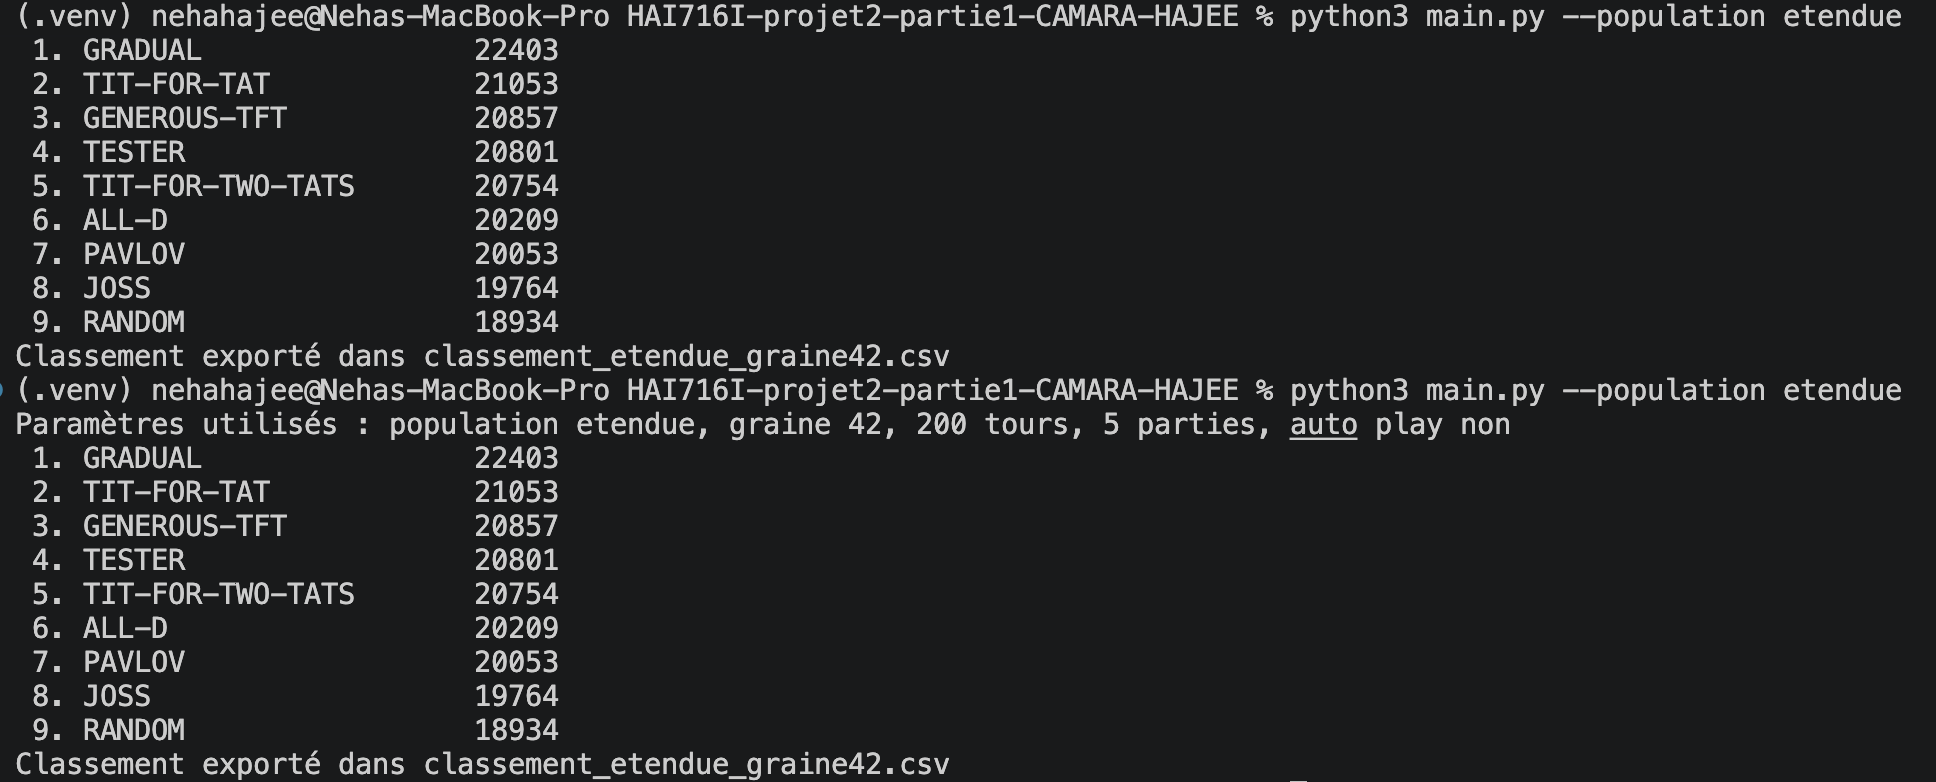
\includegraphics[width=\linewidth]{captures/etape2_classement.png}
  \caption{Deux lancements successifs de \texttt{python3 main.py --population etendue} (graine 42).}
  \label{fig:etendue}
\end{figure}

\begin{center}
\begin{tabular}{clcc}
\toprule
Rang & Stratégie & Score sans auto play & Score avec auto play \\
\midrule
1 & GRADUAL & 22403 & 25375 \\
2 & TIT-FOR-TAT & 21053 & 24146 \\
3 & GENEROUS-TFT & 20857 & 23941 \\
4 & TESTER & 20801 & 23475 \\
5 & TIT-FOR-TWO-TATS & 20754 & 23678 \\
6 & ALL-D & 20209 & 22209 \\
7 & PAVLOV & 20053 & 23136 \\
8 & JOSS & 19764 & 21991 \\
9 & RANDOM & 18934 & 21343 \\
\bottomrule
\end{tabular}
\end{center}

Le rang indiqué est celui du tournoi sans auto play. Avec auto play, l'ordre change seulement en milieu de classement,
TIT-FOR-TWO-TATS passe devant TESTER et PAVLOV passe devant ALL-D. Avec les graines 1 à 10, GRADUAL est premier et PAVLOV
septième dans les dix cas, ces résultats ne dépendent donc pas d'un tirage favorable.

Pour expliquer les écarts, les matchs de PAVLOV et de GRADUAL ont été comparés à ceux de TIT-FOR-TAT contre les mêmes
adversaires. Contre les quatre autres stratégies gentilles, les trois obtiennent 3000 points. Le tableau suivant donne les
points obtenus contre les quatre adversaires où les scores diffèrent.

\begin{center}
\begin{tabular}{lccc}
\toprule
Adversaire & TIT-FOR-TAT & GRADUAL & PAVLOV \\
\midrule
ALL-D & 1990 & 1870 & 1000 \\
RANDOM & 2498 & 3329 & 2417 \\
TESTER & 2500 & 2980 & 2335 \\
JOSS & 2065 & 2224 & 2301 \\
\midrule
Écart total avec TIT-FOR-TAT & -- & $+1350$ & $-1000$ \\
\bottomrule
\end{tabular}
\end{center}

\subsection{Analyse}
\paragraph{GRADUAL.} La prédiction est vérifiée, GRADUAL termine premier avec 1350 points d'avance sur TIT-FOR-TAT, et le
détail des matchs confirme les raisons avancées. Contre ALL-D, GRADUAL perd 120 points par rapport à TIT-FOR-TAT, et son score
de 1870, soit 374 points par partie, correspond exactement au calcul fait à la main. Contre TESTER, la coopération complète est
retrouvée après trois tours, ce qui rapporte 480 points de plus que l'écho de TIT-FOR-TAT. Le plus gros gain vient de RANDOM,
avec 831 points de plus, car les punitions qui s'allongent transforment GRADUAL en quasi ALL-D face à une stratégie qui trahit
souvent. Contre JOSS, le gain est plus modeste (159 points) et GRADUAL perd tout de même son match, car chaque trahison de JOSS
allonge la punition suivante, qui provoque à son tour des représailles. La phase d'apaisement limite l'écho sans le supprimer.

\paragraph{PAVLOV.} La prédiction est également vérifiée, PAVLOV termine septième, derrière TIT-FOR-TAT. Ses 1000 points de
retard viennent presque entièrement du match contre ALL-D, où elle obtient 1 point par tour comme prévu. Contre TESTER, le
cycle de trois tours apparaît bien, avec 2335 points de chaque côté contre 2500 pour TIT-FOR-TAT. Une partie de la prédiction
est en revanche fausse, puisque contre JOSS, PAVLOV fait mieux que TIT-FOR-TAT (2301 contre 2065). JOSS ne transforme que des
C en D, jamais l'inverse. Une fois que TIT-FOR-TAT et JOSS ont trahi tous les deux, chacun recopie le D de l'autre et la
partie reste bloquée en (D, D) jusqu'à la fin, à 2 points par tour. PAVLOV, au contraire, ne reste jamais dans (D, D), qui lui
rapporte 2, elle change donc de coup et repropose C. Elle reste ainsi dans le cycle à 2,33 points par tour. L'erreur de
prédiction vient d'une comparaison avec l'écho entre TIT-FOR-TAT et TESTER, alors que contre JOSS, TIT-FOR-TAT finit dans une
situation encore moins favorable. Enfin, avec l'auto play, PAVLOV passe devant ALL-D, ce qui va dans le sens de la prédiction
selon laquelle elle progresse quand la population contient davantage de stratégies gentilles.

\paragraph{Comparaison avec l'étape 1.} L'ajout de quatre stratégies gentilles change complètement le classement. ALL-D,
premier à l'étape 1, tombe à la sixième place. Contre les nouvelles stratégies qui ripostent, il ne gagne qu'environ 2 points
par tour, alors que ces stratégies coopèrent entre elles à 3 points par tour. Il ne profite vraiment que de PAVLOV (3500
points) et de GENEROUS-TFT (3002 points), qui se laissent exploiter. TIT-FOR-TAT remonte à la deuxième place, ce qui confirme
l'explication donnée à l'étape 1, selon laquelle la victoire d'ALL-D venait d'une population trop petite et trop peu
coopérative. Le résultat d'Axelrod, selon lequel les stratégies gentilles qui ripostent l'emportent, réapparaît dès que la
population contient suffisamment de stratégies gentilles, et GRADUAL, qui riposte de façon proportionnée et pardonne, fait
mieux que TIT-FOR-TAT.

\section{Étape 3 -- Modification du tournoi}
\subsection{Prédiction}
\subsection{Résultats}
\subsection{Analyse}

\section{Difficultés rencontrées}
\paragraph{Confusion entre scores et coups dans \texttt{jouer\_match}.} Une première version de cette fonction, après avoir
récupéré le résultat de chaque partie, le relisait dans la matrice des gains, comme dans \texttt{jouer\_partie}, en confondant
les scores d'une partie avec des coups. Le test \og toujours C contre toujours D \fg{} a provoqué une erreur
(\texttt{KeyError: (0, 1000)}) au lieu du résultat attendu (0, 5000). La correction repose sur le fait que la matrice ne sert
qu'à l'intérieur d'une partie, pour transformer deux coups en deux gains. \texttt{jouer\_partie} renvoie déjà des points, qu'il
suffit d'additionner. Cette erreur montre l'intérêt de tester chaque fonction avec des valeurs calculées à la main.

\paragraph{Simultanéité des coups dans les tests de GRADUAL.} Une première version du test de \texttt{reset} échouait. Le
script adverse ne contenait que deux coups, C puis D, et la punition était supposée déjà en cours. Or, les coups étant
simultanés, GRADUAL ne voit la trahison du deuxième tour qu'au moment de jouer le troisième. Le script a été allongé à trois
coups. Cette erreur montre que la règle de simultanéité décidée pour le moteur doit aussi être prise en compte en écrivant les
tests des stratégies.

\section{Bilan}

\end{document}
